\chapter{Data Processing}

\section{Extraction}\label{extraction}
The data for this report is an image of a coronal section of a normal brain and a brain with CTE, published by a team from the Boston University CTE Center and Brain Bank in \cite[Fig. 1]{stern2011}.
\\\\
The brain with CTE is from a retired professional (American) football player, and whilst \cite[Fig. 1]{stern2011} do not detail the patient of the control brain, we assume that it came from someone of the same sex and age at death as the CTE brain, as this is `best practice' in the field.
\\\\
We extracted the figure from the publication PDF file using an online tool. \cite{pdf24_extract_images} The extracted JPEG file is in \cref{fig:myimage}.

\begin{figure}[htbp]
  \centering
  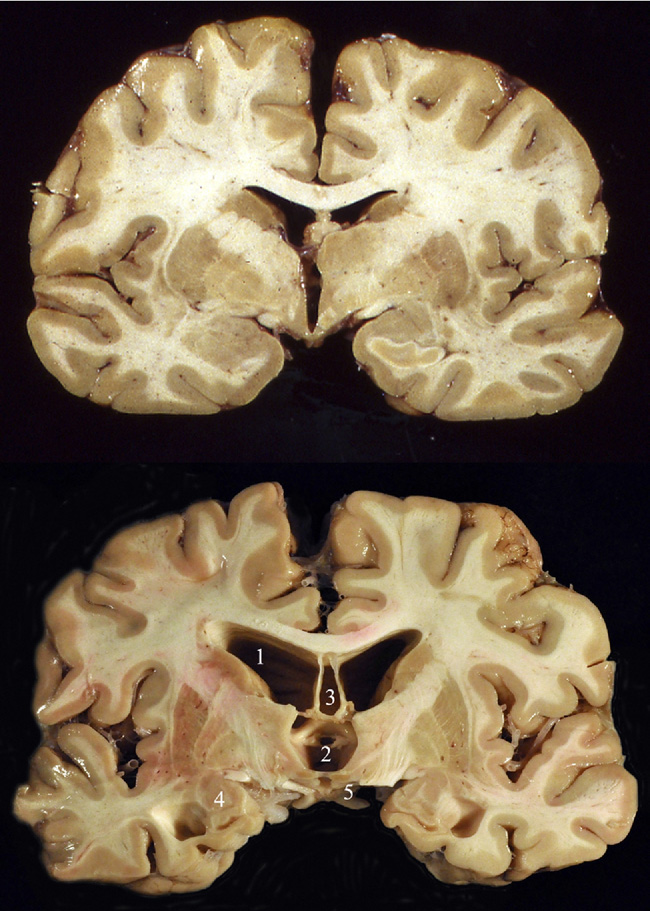
\includegraphics[width=0.4\textwidth]{extraction.jpg}
  \caption{Extraction of \cite[Fig. 1]{stern2011}.}
  \label{fig:myimage}
\end{figure}

\section{Pre-Processing}\label{preproc}
We performed two steps of pre-processing in Adobe Express Online. \cite{adobe_express_image_editor}
\begin{enumerate}
    \item \cref{fig:myimage} was cropped into two separate images.
    \item The authors of \cite{stern2011} annotated the CTE brain with numbers for use in-text. We used Adobe's \textit{wand} tool to remove the annotations.
\end{enumerate}

\section{Processing}\label{proc}
We processed the images in Python. The goal of processing was to convert the images from JPEG files to point clouds for use in TDA.
\\\\
Firstly, we rendered the images in grayscale. This decision was made pragmatically, and the limitations are discussed in \cref{limitations}.
\\\\
Secondly, we converted the grayscale image to a point cloud by a simple thresholding procedure. For each pixel in the image, a point was added to the point cloud if its brightness was greater than a certain value. We arbitrarily chose the threshold of 0.5, on a $[0,1]$ scale. The limitations of this decision are discussed in \cref{limitations}.
\\\\
Thirdly, we randomly sampled 1000 points of the point cloud. Sampling was necessary to keep computational time and RAM allocation under control, and 1000 points was the greatest number of points that did not crash the program.
\\\\
These three steps, for the control and CTE brain, are presented in \cref{fig:main}.

\begin{figure}[htbp]
  \centering
  \begin{subfigure}[b]{\textwidth}
    \centering
    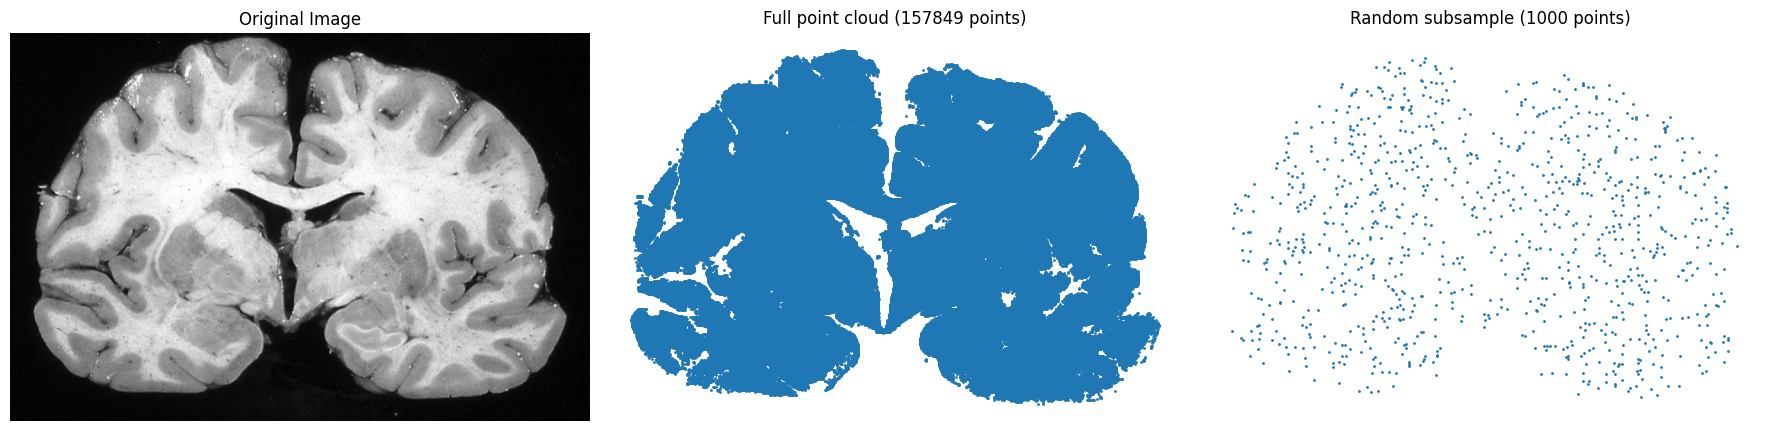
\includegraphics[width=\linewidth]{control_pointcloud.png}
    \caption{Grayscale image, full point cloud, and sampled point cloud of the control brain.}
    \label{fig:first}
  \end{subfigure}

  \vspace{1em}

  \begin{subfigure}[b]{\textwidth}
    \centering
    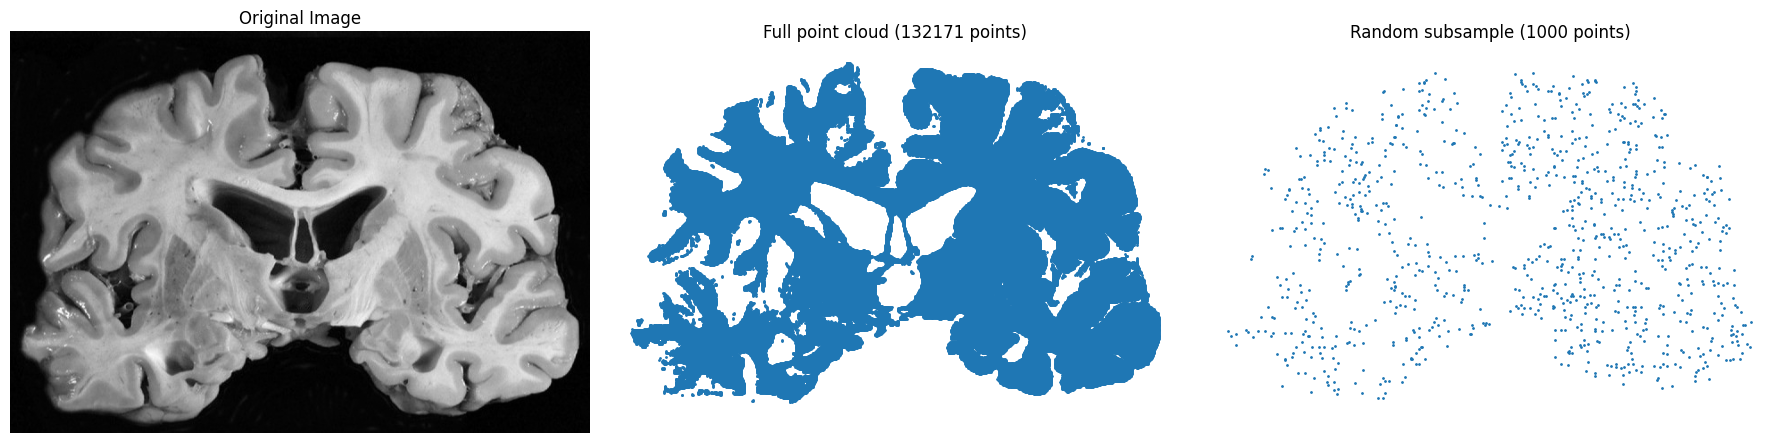
\includegraphics[width=\linewidth]{cte_pointcloud.png}
    \caption{Grayscale image, full point cloud, and sampled point cloud of the CTE brain.}
    \label{fig:second}
  \end{subfigure}

  \caption{Visualisation of data processing steps.}
  \label{fig:main}
\end{figure}